\chapter{Resultados}
\label{cap:resultados}

A análise detalhada do modelo desenvolvido é fundamental, pois a recuperação precisa de galáxias impacta diretamente na qualidade das análises científicas e na descoberta de fenômenos raros. Além disso, ao medir quantitativamente o desempenho, é possível identificar limitações, realizar ajustes ou refinar o processo de geração dos embeddings do modelo para otimizar sua aplicação em levantamentos astronômicos de larga escala.

Neste capítulo, será feita a avaliação do modelo no conjunto de teste para as tarefas de simulação dos votos (Seção \ref{sec:res-teste}) e recuperação de imagens a partir das representações visuais (Seção \ref{sec:res-ret}), por fim, também é feita uma avaliação de usabilidade do sistema (Seção \ref{sec:res-sist}).


% \section{Avaliação do Treinamento do Modelo}
% \label{sec:res-treinamento}



\section{Avaliação do Modelo no Conjunto de Teste}
\label{sec:res-teste}

A análise quantitativa das métricas de desempenho no conjunto de teste é fundamental para avaliar a capacidade preditiva e de generalização de um modelo de aprendizado profundo. A Tabela \ref{tab:test-metrics} sumariza as métricas de acurácia (Seção \ref{sec:metricas-acc}), precisão (Seção \ref{sec:metricas-precisao}), revocação (Seção \ref{sec:metricas-revocacao}) e F1-score (Seção \ref{sec:metricas-f1}) para várias perguntas do GalaxyZoo.

\begin{table}[!ht]
  \centering
  \caption{Avaliação do modelo no conjunto de teste}
  \label{tab:test-metrics}
  \begin{tabular}{lcccc}
    \toprule
    Questão            & Acurácia & Precisão & Revocação & F1       \\
    \midrule
    Spiral winding     & 0.833771 & 0.714138 & 0.717103  & 0.715594 \\
    Bar                & 0.890751 & 0.715289 & 0.780659  & 0.742811 \\
    Edge on bulge      & 0.943199 & 0.817953 & 0.895207  & 0.851695 \\
    Disk edge on       & 0.973585 & 0.969010 & 0.970718  & 0.969856 \\
    Smooth or featured & 0.974996 & -        & -         & -        \\
    Has spiral arms    & 0.942789 & 0.898665 & 0.859011  & 0.877276 \\
    Galaxy Symetrical  & 0.980000 & 0.973438 & 0.966997  & 0.970173 \\
    Clumpy appearence  & 0.962085 & 0.956045 & 0.958264  & 0.957141 \\
    How rounded        & 0.952254 & 0.919239 & 0.927339  & 0.923121 \\
    Merging            & 0.981400 & 0.666607 & 0.771892  & 0.703503 \\
    Bulge size         & 0.931864 & 0.683324 & 0.734342  & 0.701055 \\
    Spiral arms count  & 0.954545 & 0.684281 & 0.758884  & 0.716117 \\
    \bottomrule
  \end{tabular}
\end{table}

Para dar continuidade na avaliação quantitativa no conjunto de teste, a seguir, são mostradas as matrizes de confusão (Seção \ref{sec:metricas-confusao}) para questão da Tabela \ref{tab:test-metrics}.


\begin{figure}[!ht]
  \centering
  \caption{Matrizes de confusão para cada questão no conjunto de teste}
  \label{fig:cm_1}
  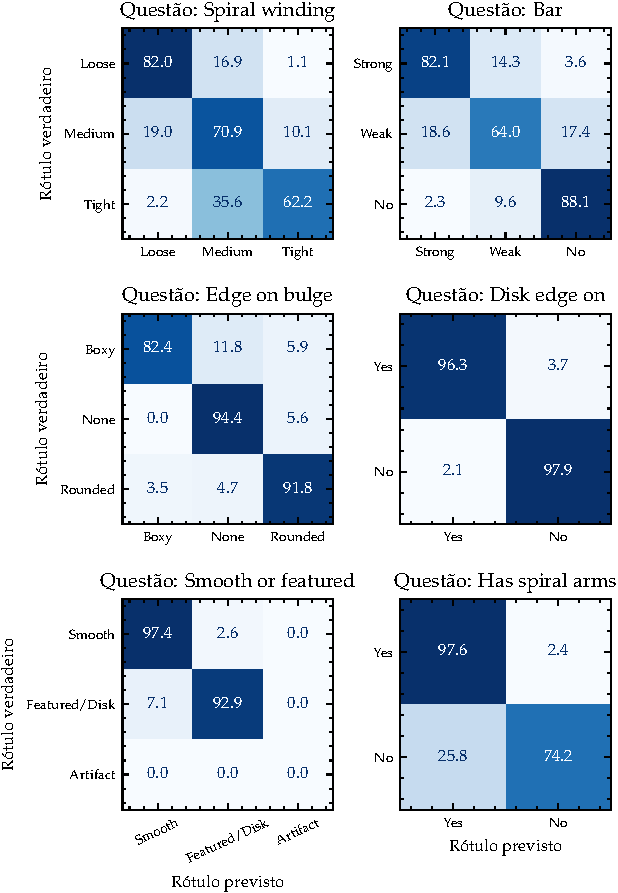
\includegraphics[width=\linewidth]{notebooks/plots/cm_1.pdf}
\end{figure}

\begin{figure}[!ht]
  \centering
  \caption{Matrizes de confusão para cada questão no conjunto de teste (continuação)}
  \label{fig:cm_2}
  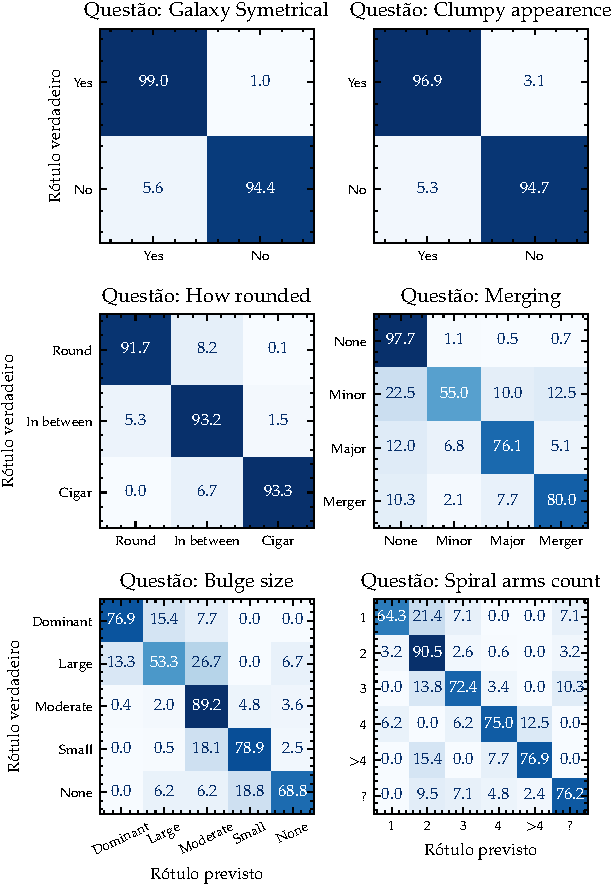
\includegraphics[width=\linewidth]{notebooks/plots/cm_2.pdf}
\end{figure}


Os velores mostrados na Tabela \ref{tab:test-metrics} e nas Figs. \ref{fig:cm_1} e \ref{fig:cm_2} mostram a eficiência do modelo em identificar as características morfológicas das galáxias. Essa análise evidencia que o modelo não apenas possui bom desempenho em dados de treinamento, mas também é capaz de generalizar para novos conjuntos de dados, aspecto crucial para aplicações científicas confiáveis.




\section{Avaliação da Recuperação de Imagens}
\label{sec:res-ret}

A avaliação quantitativa do desempenho do sistema para a tarefa de recuperação de imagens é feita utilizando a métrica mean Average Precision (mAP; Seção \ref{sec:metricas-map}), pois esta medida é crucial para avaliar a capacidade do sistema em priorizar e classificar corretamente imagens relevantes em relação a consultas específicas. A mAP integra a precisão ao longo de diferentes níveis de revocação, proporcionando uma visão detalhada do desempenho global do modelo em recuperar galáxias em grandes bancos de dados.

Os valores de mAP apresentados na Tabela \ref{tab:test-map} evidenciam a habilidade do modelo em manter alta relevância entre os itens recuperados, mesmo em cenários de grande complexidade ou com classes desbalanceadas. Essa métrica assegura que o sistema não apenas é eficaz em identificar galáxias relevantes, mas também organiza as recuperações de forma a maximizar sua utilidade científica, destacando a robustez e a capacidade de generalização do modelo para aplicações astronômicas.

\begin{table}[!ht]
  \centering
  \caption{Avaliação do modelo para tarefa de recuperação de imagens}
  \label{tab:test-map}
  \begin{tabular}{lc}
    \toprule
    Questão            & mAP      \\
    \midrule
    Spiral winding     & 0.988254 \\
    Bar                & 0.980521 \\
    Edge on bulge      & 0.990124 \\
    Disk edge on       & 0.999986 \\
    Smooth or featured & 0.987412 \\
    Has spiral arms    & 0.968340 \\
    Galaxy Symetrical  & 0.962513 \\
    Clumpy appearence  & 0.957814 \\
    How rounded        & 0.978536 \\
    Merging            & 0.963656 \\
    Bulge size         & 0.987431 \\
    Spiral arms count  & 0.960259 \\
    \bottomrule
  \end{tabular}
\end{table}


A seguir, as Figs. \ref{fig:q1}, \ref{fig:q2}, \ref{fig:q3}, \ref{fig:q4}, \ref{fig:q5}, \ref{fig:q6} e \ref{fig:q7} mostram as buscas por similaridade visual para vários tipos de galáxias com a finalidade de exemplificar os resultados das buscas por similaridade visual obtidas pelo sistema desenvolvido.


\begin{figure}[!ht]
  \centering
  \caption{Resultados da busca para a galáxia UGC 9010}
  \label{fig:q1}
  \begin{overpic}[width=0.195\linewidth]{figures/stamps/q1_0}
    \put (3, 7) {\large\color{white} Query}
  \end{overpic}
  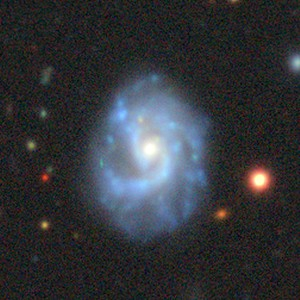
\includegraphics[width=0.195\linewidth]{figures/stamps/q1_1}
  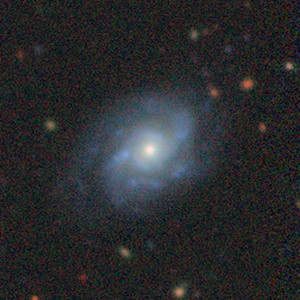
\includegraphics[width=0.195\linewidth]{figures/stamps/q1_2}
  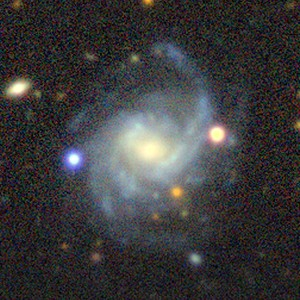
\includegraphics[width=0.195\linewidth]{figures/stamps/q1_3}
  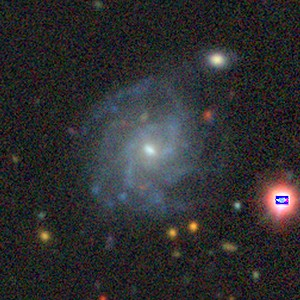
\includegraphics[width=0.195\linewidth]{figures/stamps/q1_4}\\[2mm]
  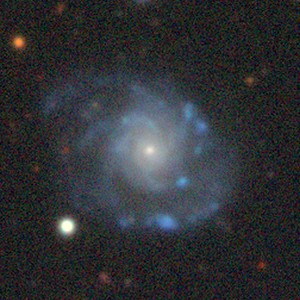
\includegraphics[width=0.195\linewidth]{figures/stamps/q1_5}
  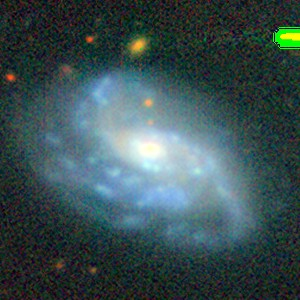
\includegraphics[width=0.195\linewidth]{figures/stamps/q1_6}
  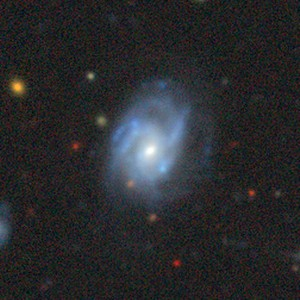
\includegraphics[width=0.195\linewidth]{figures/stamps/q1_7}
  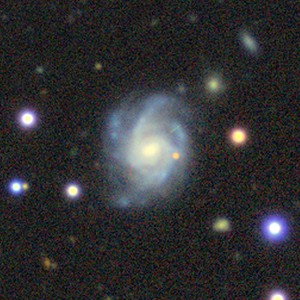
\includegraphics[width=0.195\linewidth]{figures/stamps/q1_8}
  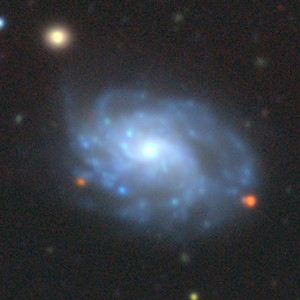
\includegraphics[width=0.195\linewidth]{figures/stamps/q1_9}\\[2mm]
  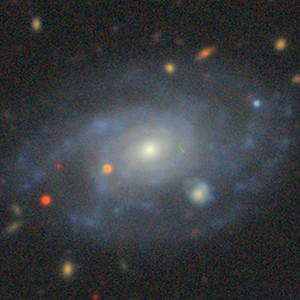
\includegraphics[width=0.195\linewidth]{figures/stamps/q1_10}
  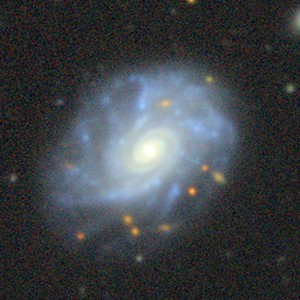
\includegraphics[width=0.195\linewidth]{figures/stamps/q1_11}
  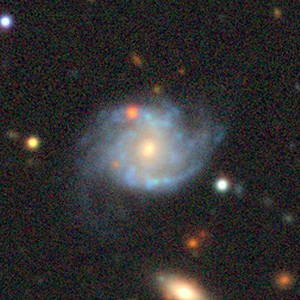
\includegraphics[width=0.195\linewidth]{figures/stamps/q1_12}
  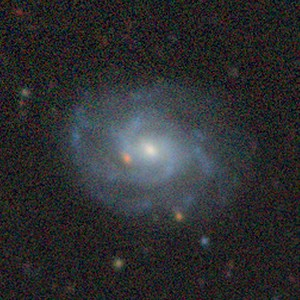
\includegraphics[width=0.195\linewidth]{figures/stamps/q1_13}
  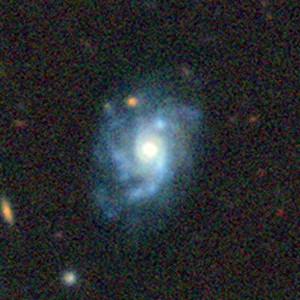
\includegraphics[width=0.195\linewidth]{figures/stamps/q1_14}\\[2mm]
  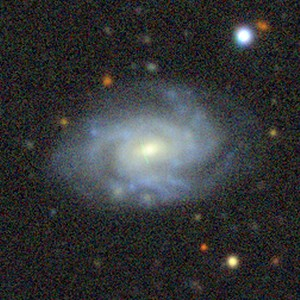
\includegraphics[width=0.195\linewidth]{figures/stamps/q1_15}
  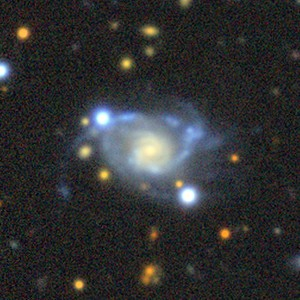
\includegraphics[width=0.195\linewidth]{figures/stamps/q1_16}
  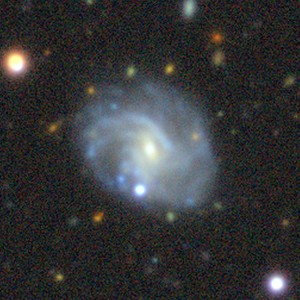
\includegraphics[width=0.195\linewidth]{figures/stamps/q1_17}
  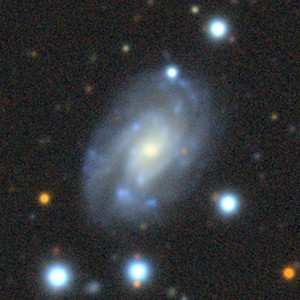
\includegraphics[width=0.195\linewidth]{figures/stamps/q1_18}
  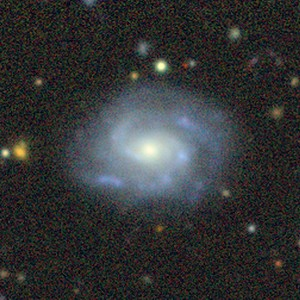
\includegraphics[width=0.195\linewidth]{figures/stamps/q1_19}\\[2mm]
  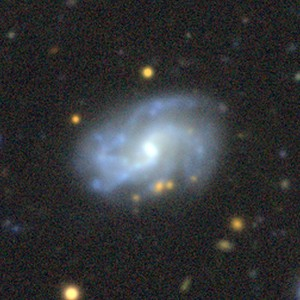
\includegraphics[width=0.195\linewidth]{figures/stamps/q1_20}
  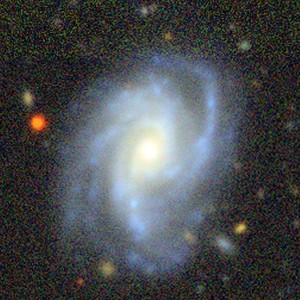
\includegraphics[width=0.195\linewidth]{figures/stamps/q1_21}
  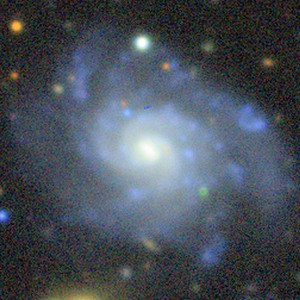
\includegraphics[width=0.195\linewidth]{figures/stamps/q1_22}
  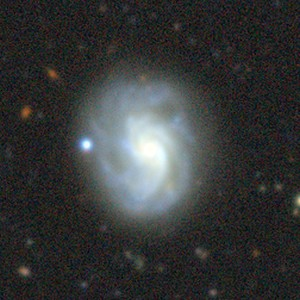
\includegraphics[width=0.195\linewidth]{figures/stamps/q1_23}
  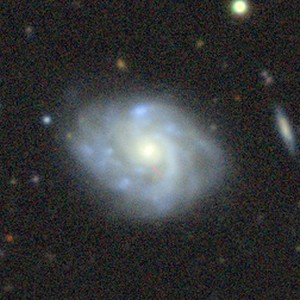
\includegraphics[width=0.195\linewidth]{figures/stamps/q1_24}\\[2mm]
  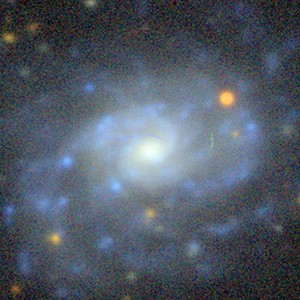
\includegraphics[width=0.195\linewidth]{figures/stamps/q1_25}
  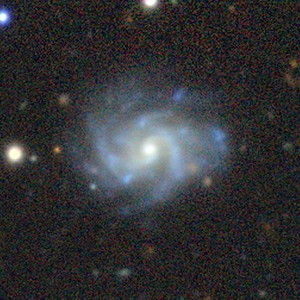
\includegraphics[width=0.195\linewidth]{figures/stamps/q1_26}
  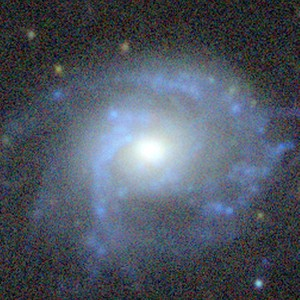
\includegraphics[width=0.195\linewidth]{figures/stamps/q1_27}
  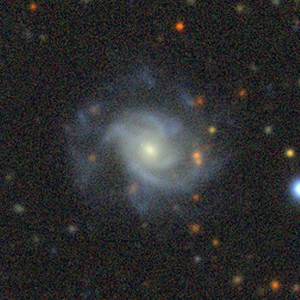
\includegraphics[width=0.195\linewidth]{figures/stamps/q1_28}
  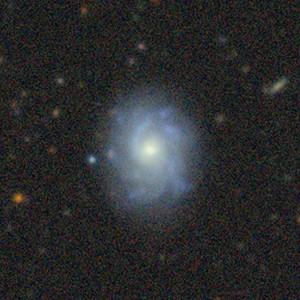
\includegraphics[width=0.195\linewidth]{figures/stamps/q1_29}
  \legend{UGC 9010 é uma galáxia espiral com orientação face-on (face para o observador). O primeiro painel (Query) mostra a imagem da galáxia UGC 9010, utilizada como referência. Os demais painéis mostram as galáxias obtidas por similaridade visual. Esta busca utilizou a distância do cosseno (Seção \ref{sec:metricas-cos}) como métrica de similaridade.}
\end{figure}


\begin{figure}[!ht]
  \centering
  \caption{Resultados da busca para a galáxia NGC 1043}
  \label{fig:q2}
  \begin{overpic}[width=0.195\linewidth]{figures/stamps/q2_0}
    \put (3, 7) {\large\color{white} Query}
  \end{overpic}
  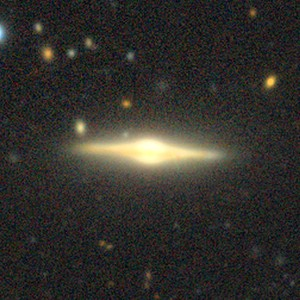
\includegraphics[width=0.195\linewidth]{figures/stamps/q2_1}
  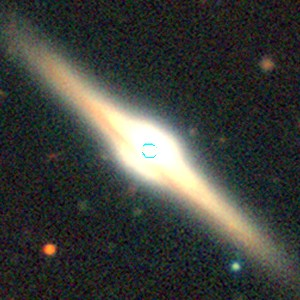
\includegraphics[width=0.195\linewidth]{figures/stamps/q2_2}
  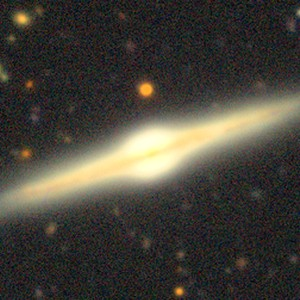
\includegraphics[width=0.195\linewidth]{figures/stamps/q2_3}
  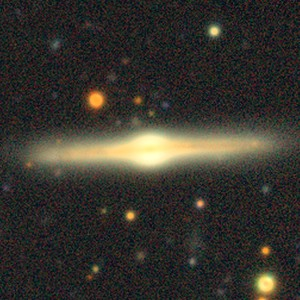
\includegraphics[width=0.195\linewidth]{figures/stamps/q2_4}\\[2mm]
  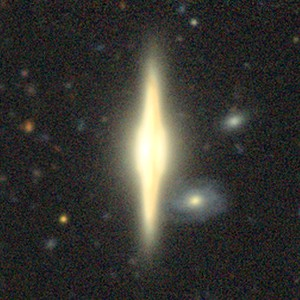
\includegraphics[width=0.195\linewidth]{figures/stamps/q2_5}
  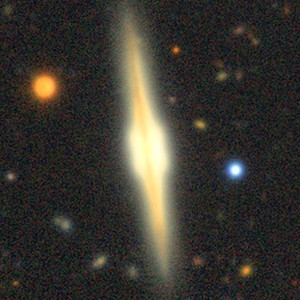
\includegraphics[width=0.195\linewidth]{figures/stamps/q2_6}
  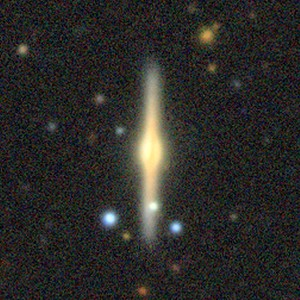
\includegraphics[width=0.195\linewidth]{figures/stamps/q2_7}
  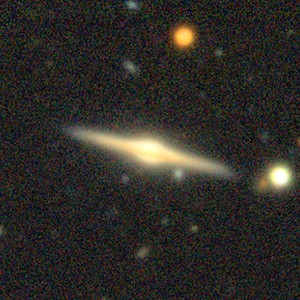
\includegraphics[width=0.195\linewidth]{figures/stamps/q2_8}
  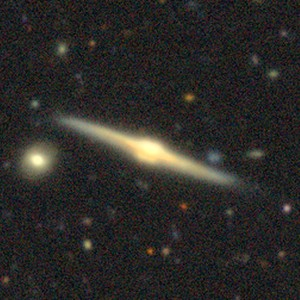
\includegraphics[width=0.195\linewidth]{figures/stamps/q2_9}\\[2mm]
  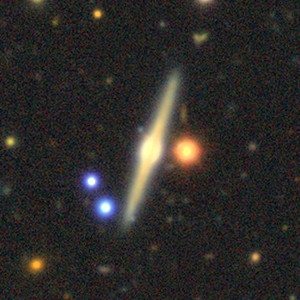
\includegraphics[width=0.195\linewidth]{figures/stamps/q2_10}
  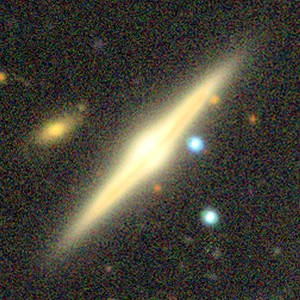
\includegraphics[width=0.195\linewidth]{figures/stamps/q2_11}
  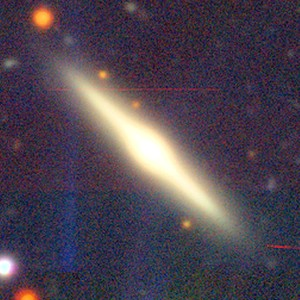
\includegraphics[width=0.195\linewidth]{figures/stamps/q2_12}
  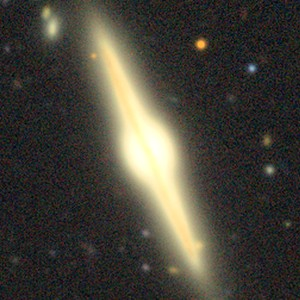
\includegraphics[width=0.195\linewidth]{figures/stamps/q2_13}
  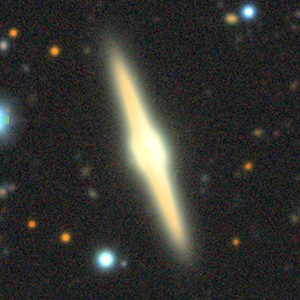
\includegraphics[width=0.195\linewidth]{figures/stamps/q2_14}\\[2mm]
  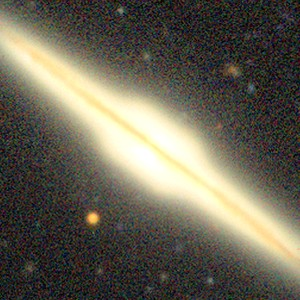
\includegraphics[width=0.195\linewidth]{figures/stamps/q2_15}
  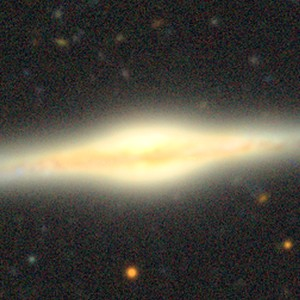
\includegraphics[width=0.195\linewidth]{figures/stamps/q2_16}
  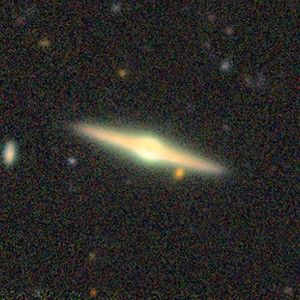
\includegraphics[width=0.195\linewidth]{figures/stamps/q2_17}
  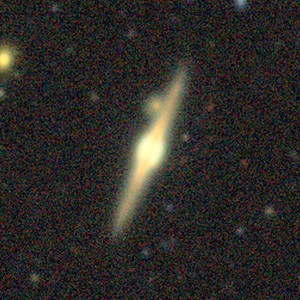
\includegraphics[width=0.195\linewidth]{figures/stamps/q2_18}
  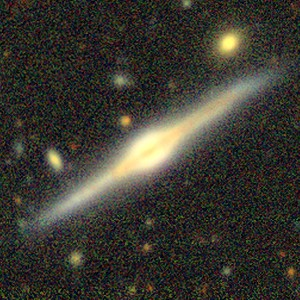
\includegraphics[width=0.195\linewidth]{figures/stamps/q2_19}\\[2mm]
  \includegraphics[width=0.195\linewidth]{figures/stamps/q2_20}
  \includegraphics[width=0.195\linewidth]{figures/stamps/q2_21}
  \includegraphics[width=0.195\linewidth]{figures/stamps/q2_22}
  \includegraphics[width=0.195\linewidth]{figures/stamps/q2_23}
  \includegraphics[width=0.195\linewidth]{figures/stamps/q2_24}\\[2mm]
  \includegraphics[width=0.195\linewidth]{figures/stamps/q2_25}
  \includegraphics[width=0.195\linewidth]{figures/stamps/q2_26}
  \includegraphics[width=0.195\linewidth]{figures/stamps/q2_27}
  \includegraphics[width=0.195\linewidth]{figures/stamps/q2_28}
  \includegraphics[width=0.195\linewidth]{figures/stamps/q2_29}
  \legend{NGC 1043 é uma galáxia espiral com orientação edge-on (borda para o observador). O primeiro painel (Query) mostra a imagem da galáxia NGC 1043, utilizada como referência. Os demais painéis mostram as galáxias obtidas por similaridade visual. Esta busca utilizou a distância do cosseno (Seção \ref{sec:metricas-cos}) como métrica de similaridade.}
\end{figure}



\begin{figure}[!ht]
  \centering
  \caption{Resultados da busca para a galáxia J082404.58+315023.3}
  \label{fig:q3}
  \begin{overpic}[width=0.195\linewidth]{figures/stamps/q3_0}
    \put (3, 7) {\large\color{white} Query}
  \end{overpic}
  \includegraphics[width=0.195\linewidth]{figures/stamps/q3_1}
  \includegraphics[width=0.195\linewidth]{figures/stamps/q3_2}
  \includegraphics[width=0.195\linewidth]{figures/stamps/q3_3}
  \includegraphics[width=0.195\linewidth]{figures/stamps/q3_4}\\[2mm]
  \includegraphics[width=0.195\linewidth]{figures/stamps/q3_5}
  \includegraphics[width=0.195\linewidth]{figures/stamps/q3_6}
  \includegraphics[width=0.195\linewidth]{figures/stamps/q3_7}
  \includegraphics[width=0.195\linewidth]{figures/stamps/q3_8}
  \includegraphics[width=0.195\linewidth]{figures/stamps/q3_9}\\[2mm]
  \includegraphics[width=0.195\linewidth]{figures/stamps/q3_10}
  \includegraphics[width=0.195\linewidth]{figures/stamps/q3_11}
  \includegraphics[width=0.195\linewidth]{figures/stamps/q3_12}
  \includegraphics[width=0.195\linewidth]{figures/stamps/q3_13}
  \includegraphics[width=0.195\linewidth]{figures/stamps/q3_14}\\[2mm]
  \includegraphics[width=0.195\linewidth]{figures/stamps/q3_15}
  \includegraphics[width=0.195\linewidth]{figures/stamps/q3_16}
  \includegraphics[width=0.195\linewidth]{figures/stamps/q3_17}
  \includegraphics[width=0.195\linewidth]{figures/stamps/q3_18}
  \includegraphics[width=0.195\linewidth]{figures/stamps/q3_19}\\[2mm]
  \includegraphics[width=0.195\linewidth]{figures/stamps/q3_20}
  \includegraphics[width=0.195\linewidth]{figures/stamps/q3_21}
  \includegraphics[width=0.195\linewidth]{figures/stamps/q3_22}
  \includegraphics[width=0.195\linewidth]{figures/stamps/q3_23}
  \includegraphics[width=0.195\linewidth]{figures/stamps/q3_24}\\[2mm]
  \includegraphics[width=0.195\linewidth]{figures/stamps/q3_25}
  \includegraphics[width=0.195\linewidth]{figures/stamps/q3_26}
  \includegraphics[width=0.195\linewidth]{figures/stamps/q3_27}
  \includegraphics[width=0.195\linewidth]{figures/stamps/q3_28}
  \includegraphics[width=0.195\linewidth]{figures/stamps/q3_29}
  \legend{J082404.58+315023.3 é uma galáxia compacta, sua ocorrência na natureza é extremamente rara. O primeiro painel (Query) mostra a imagem da galáxia J082404.58+315023.3, utilizada como referência. Os demais painéis mostram as galáxias obtidas por similaridade visual. Esta busca utilizou a distância do cosseno (Seção \ref{sec:metricas-cos}) como métrica de similaridade.}
\end{figure}



\begin{figure}[!ht]
  \centering
  \caption{Resultados da busca para a galáxia UGC 1698}
  \label{fig:q4}
  \begin{overpic}[width=0.195\linewidth]{figures/stamps/q4_0}
    \put (3, 7) {\large\color{white} Query}
  \end{overpic}
  \includegraphics[width=0.195\linewidth]{figures/stamps/q4_1}
  \includegraphics[width=0.195\linewidth]{figures/stamps/q4_7}
  \includegraphics[width=0.195\linewidth]{figures/stamps/q4_3}
  \includegraphics[width=0.195\linewidth]{figures/stamps/q4_4}\\[2mm]
  \includegraphics[width=0.195\linewidth]{figures/stamps/q4_5}
  \includegraphics[width=0.195\linewidth]{figures/stamps/q4_6}
  \includegraphics[width=0.195\linewidth]{figures/stamps/q4_2}
  \includegraphics[width=0.195\linewidth]{figures/stamps/q4_8}
  \includegraphics[width=0.195\linewidth]{figures/stamps/q4_9}\\[2mm]
  \includegraphics[width=0.195\linewidth]{figures/stamps/q4_10}
  \includegraphics[width=0.195\linewidth]{figures/stamps/q4_11}
  \includegraphics[width=0.195\linewidth]{figures/stamps/q4_12}
  \includegraphics[width=0.195\linewidth]{figures/stamps/q4_21}
  \includegraphics[width=0.195\linewidth]{figures/stamps/q4_14}\\[2mm]
  \includegraphics[width=0.195\linewidth]{figures/stamps/q4_15}
  \includegraphics[width=0.195\linewidth]{figures/stamps/q4_16}
  \includegraphics[width=0.195\linewidth]{figures/stamps/q4_17}
  \includegraphics[width=0.195\linewidth]{figures/stamps/q4_18}
  \includegraphics[width=0.195\linewidth]{figures/stamps/q4_19}\\[2mm]
  \includegraphics[width=0.195\linewidth]{figures/stamps/q4_20}
  \includegraphics[width=0.195\linewidth]{figures/stamps/q4_13}
  \includegraphics[width=0.195\linewidth]{figures/stamps/q4_22}
  \includegraphics[width=0.195\linewidth]{figures/stamps/q4_23}
  \includegraphics[width=0.195\linewidth]{figures/stamps/q4_24}\\[2mm]
  \includegraphics[width=0.195\linewidth]{figures/stamps/q4_25}
  \includegraphics[width=0.195\linewidth]{figures/stamps/q4_26}
  \includegraphics[width=0.195\linewidth]{figures/stamps/q4_27}
  \includegraphics[width=0.195\linewidth]{figures/stamps/q4_28}
  \includegraphics[width=0.195\linewidth]{figures/stamps/q4_29}
  \legend{UGC 1698 é uma espiral barrada, o sistema foi capaz de recuperar galáxias muito parecidas. O primeiro painel (Query) mostra a imagem da galáxia UGC 1698, utilizada como referência. Os demais painéis mostram as galáxias obtidas por similaridade visual. Esta busca utilizou a distância do cosseno (Seção \ref{sec:metricas-cos}) como métrica de similaridade.}
\end{figure}





\begin{figure}[!ht]
  \centering
  \caption{Resultados da busca para a galáxia J060430.95-470755.7}
  \label{fig:q5}
  \begin{overpic}[width=0.195\linewidth]{figures/stamps/q5_0}
    \put (3, 7) {\large\color{white} Query}
  \end{overpic}
  \includegraphics[width=0.195\linewidth]{figures/stamps/q5_1}
  \includegraphics[width=0.195\linewidth]{figures/stamps/q5_2}
  \includegraphics[width=0.195\linewidth]{figures/stamps/q5_3}
  \includegraphics[width=0.195\linewidth]{figures/stamps/q5_4}\\[2mm]
  \includegraphics[width=0.195\linewidth]{figures/stamps/q5_5}
  \includegraphics[width=0.195\linewidth]{figures/stamps/q5_6}
  \includegraphics[width=0.195\linewidth]{figures/stamps/q5_7}
  \includegraphics[width=0.195\linewidth]{figures/stamps/q5_8}
  \includegraphics[width=0.195\linewidth]{figures/stamps/q5_9}\\[2mm]
  \includegraphics[width=0.195\linewidth]{figures/stamps/q5_10}
  \includegraphics[width=0.195\linewidth]{figures/stamps/q5_11}
  \includegraphics[width=0.195\linewidth]{figures/stamps/q5_12}
  \includegraphics[width=0.195\linewidth]{figures/stamps/q5_13}
  \includegraphics[width=0.195\linewidth]{figures/stamps/q5_14}\\[2mm]
  \includegraphics[width=0.195\linewidth]{figures/stamps/q5_15}
  \includegraphics[width=0.195\linewidth]{figures/stamps/q5_16}
  \includegraphics[width=0.195\linewidth]{figures/stamps/q5_17}
  \includegraphics[width=0.195\linewidth]{figures/stamps/q5_18}
  \includegraphics[width=0.195\linewidth]{figures/stamps/q5_19}\\[2mm]
  \includegraphics[width=0.195\linewidth]{figures/stamps/q5_20}
  \includegraphics[width=0.195\linewidth]{figures/stamps/q5_21}
  \includegraphics[width=0.195\linewidth]{figures/stamps/q5_22}
  \includegraphics[width=0.195\linewidth]{figures/stamps/q5_23}
  \includegraphics[width=0.195\linewidth]{figures/stamps/q5_24}\\[2mm]
  \includegraphics[width=0.195\linewidth]{figures/stamps/q5_25}
  \includegraphics[width=0.195\linewidth]{figures/stamps/q5_26}
  \includegraphics[width=0.195\linewidth]{figures/stamps/q5_27}
  \includegraphics[width=0.195\linewidth]{figures/stamps/q5_28}
  \includegraphics[width=0.195\linewidth]{figures/stamps/q5_29}
  \legend{J060430.95-470755.7 é uma galáxia com enrolamento dos braços espirais abertos. O primeiro painel (Query) mostra a imagem da galáxia J060430.95-470755.7, utilizada como referência. Os demais painéis mostram as galáxias obtidas por similaridade visual. Esta busca utilizou a distância do cosseno (Seção \ref{sec:metricas-cos}) como métrica de similaridade.}
\end{figure}




\begin{figure}[!ht]
  \centering
  \caption{Resultados da busca para a galáxia UGC 767}
  \label{fig:q6}
  \begin{overpic}[width=0.195\linewidth]{figures/stamps/q6_0}
    \put (3, 7) {\large\color{white} Query}
  \end{overpic}
  \includegraphics[width=0.195\linewidth]{figures/stamps/q6_1}
  \includegraphics[width=0.195\linewidth]{figures/stamps/q6_2}
  \includegraphics[width=0.195\linewidth]{figures/stamps/q6_3}
  \includegraphics[width=0.195\linewidth]{figures/stamps/q6_4}\\[2mm]
  \includegraphics[width=0.195\linewidth]{figures/stamps/q6_5}
  \includegraphics[width=0.195\linewidth]{figures/stamps/q6_6}
  \includegraphics[width=0.195\linewidth]{figures/stamps/q6_7}
  \includegraphics[width=0.195\linewidth]{figures/stamps/q6_8}
  \includegraphics[width=0.195\linewidth]{figures/stamps/q6_9}\\[2mm]
  \includegraphics[width=0.195\linewidth]{figures/stamps/q6_10}
  \includegraphics[width=0.195\linewidth]{figures/stamps/q6_11}
  \includegraphics[width=0.195\linewidth]{figures/stamps/q6_12}
  \includegraphics[width=0.195\linewidth]{figures/stamps/q6_13}
  \includegraphics[width=0.195\linewidth]{figures/stamps/q6_14}\\[2mm]
  \includegraphics[width=0.195\linewidth]{figures/stamps/q6_15}
  \includegraphics[width=0.195\linewidth]{figures/stamps/q6_16}
  \includegraphics[width=0.195\linewidth]{figures/stamps/q6_17}
  \includegraphics[width=0.195\linewidth]{figures/stamps/q6_18}
  \includegraphics[width=0.195\linewidth]{figures/stamps/q6_19}\\[2mm]
  \includegraphics[width=0.195\linewidth]{figures/stamps/q6_20}
  \includegraphics[width=0.195\linewidth]{figures/stamps/q6_21}
  \includegraphics[width=0.195\linewidth]{figures/stamps/q6_22}
  \includegraphics[width=0.195\linewidth]{figures/stamps/q6_23}
  \includegraphics[width=0.195\linewidth]{figures/stamps/q6_24}\\[2mm]
  \includegraphics[width=0.195\linewidth]{figures/stamps/q6_25}
  \includegraphics[width=0.195\linewidth]{figures/stamps/q6_26}
  \includegraphics[width=0.195\linewidth]{figures/stamps/q6_27}
  \includegraphics[width=0.195\linewidth]{figures/stamps/q6_28}
  \includegraphics[width=0.195\linewidth]{figures/stamps/q6_29}
  \legend{UGC 767 é uma galáxia elíptica. O primeiro painel (Query) mostra a imagem da galáxia UGC 767, utilizada como referência. Os demais painéis mostram as galáxias obtidas por similaridade visual. Esta busca utilizou a distância do cosseno (Seção \ref{sec:metricas-cos}) como métrica de similaridade.}
\end{figure}



\begin{figure}[!ht]
  \centering
  \caption{Resultados da busca para a galáxia J151806.13+424445.2}
  \label{fig:q7}
  \begin{overpic}[width=0.195\linewidth]{figures/stamps/q7_0}
    \put (3, 7) {\large\color{white} Query}
  \end{overpic}
  \includegraphics[width=0.195\linewidth]{figures/stamps/q7_1}
  \includegraphics[width=0.195\linewidth]{figures/stamps/q7_2}
  \includegraphics[width=0.195\linewidth]{figures/stamps/q7_3}
  \includegraphics[width=0.195\linewidth]{figures/stamps/q7_4}\\[2mm]
  \includegraphics[width=0.195\linewidth]{figures/stamps/q7_5}
  \includegraphics[width=0.195\linewidth]{figures/stamps/q7_6}
  \includegraphics[width=0.195\linewidth]{figures/stamps/q7_7}
  \includegraphics[width=0.195\linewidth]{figures/stamps/q7_8}
  \includegraphics[width=0.195\linewidth]{figures/stamps/q7_9}\\[2mm]
  \includegraphics[width=0.195\linewidth]{figures/stamps/q7_10}
  \includegraphics[width=0.195\linewidth]{figures/stamps/q7_11}
  \includegraphics[width=0.195\linewidth]{figures/stamps/q7_12}
  \includegraphics[width=0.195\linewidth]{figures/stamps/q7_13}
  \includegraphics[width=0.195\linewidth]{figures/stamps/q7_14}\\[2mm]
  \includegraphics[width=0.195\linewidth]{figures/stamps/q7_15}
  \includegraphics[width=0.195\linewidth]{figures/stamps/q7_16}
  \includegraphics[width=0.195\linewidth]{figures/stamps/q7_17}
  \includegraphics[width=0.195\linewidth]{figures/stamps/q7_18}
  \includegraphics[width=0.195\linewidth]{figures/stamps/q7_19}\\[2mm]
  \includegraphics[width=0.195\linewidth]{figures/stamps/q7_20}
  \includegraphics[width=0.195\linewidth]{figures/stamps/q7_21}
  \includegraphics[width=0.195\linewidth]{figures/stamps/q7_22}
  \includegraphics[width=0.195\linewidth]{figures/stamps/q7_23}
  \includegraphics[width=0.195\linewidth]{figures/stamps/q7_24}\\[2mm]
  \includegraphics[width=0.195\linewidth]{figures/stamps/q7_25}
  \includegraphics[width=0.195\linewidth]{figures/stamps/q7_26}
  \includegraphics[width=0.195\linewidth]{figures/stamps/q7_27}
  \includegraphics[width=0.195\linewidth]{figures/stamps/q7_28}
  \includegraphics[width=0.195\linewidth]{figures/stamps/q7_29}
  \legend{J151806.13+424445.2 mostra um fenômeno raro de fusão de duas galáxias. O primeiro painel (Query) mostra a imagem da galáxia J151806.13+424445.2, utilizada como referência. Os demais painéis mostram as galáxias obtidas por similaridade visual. Esta busca utilizou a distância do cosseno (Seção \ref{sec:metricas-cos}) como métrica de similaridade.}
\end{figure}



\section{Avaliação do Sistema de Informação}
\label{sec:res-sist}

Na avaliação do Sistema de Informação, são considerados aspectos fundamentais para garantir uma alta experiência de usuário, como o tempo gasto para executar cada tarefa (Seção \ref{sec:sist-performance}) e os aspectos de interface com o usuário (Seção \ref{sec:sist-ui}).


\subsection{Performance}
\label{sec:sist-performance}

A performance relacionada ao tempo de busca do sistema inteligente é fundamental para garantir sua viabilidade prática, especialmente diante do crescente volume de dados provenientes de levantamentos astronômicos de larga escala. Um tempo de busca otimizado garante a eficiência na recuperação de imagens relevantes, permitindo que pesquisadores obtenham resultados em tempo hábil para análises científicas. Isso é particularmente crítico em contextos como o monitoramento de eventos astronômicos transitórios, onde a agilidade na identificação de padrões visuais similares pode influenciar descobertas e reações rápidas.

A Tabela \ref{tab:times} sumariza o tempo gasto em cada etapa da busca. As otimizações implementadas na base de dados (Seções \ref{sec:si-coords-index} e \ref{sec:si-vec-index}) a partir de índices específicos para cada tipo de dado colaboram para o desempenho da busca. No entanto, a maior parte do tempo é gasto na resolução do objeto, não sendo possível mitigá-lo, pois é realizado em um serviço na núvem externo. Este foi o principal motivo para implementar o sistema de cache.

% Além disso, tempos de busca reduzidos refletem uma arquitetura eficiente, incluindo o uso de embeddings compactos e estruturas de indexação, como árvores k-d ou grafos aproximados, que possibilitam escalabilidade sem comprometer a precisão da recuperação. Assim, a avaliação da performance temporal é essencial para assegurar que o sistema seja útil tanto em termos de resposta imediata quanto de processamento em larga escala.

\begin{table}[!ht]
  \centering
  \caption{Tempo gasto nas tarefas executadas durante a busca}
  \label{tab:times}
  \begin{tabular}{lcc}
    \toprule
    Tarefa            & Tempo gasto (sem cache) & Tempo gasto (com cache) \\
    \midrule
    Resolução do nome & $4.3 \pm 2.8$           & $0.1 \pm 0.0$           \\
    Busca em cone     & $1.7 \pm 0.8$           & $0.0 \pm 0.0$           \\
    Busca vetorial    & $2.1 \pm 0.9$           & $0.1 \pm 0.0$           \\
    \bottomrule
  \end{tabular}
\end{table}



\subsection{Interface Gráfica}
\label{sec:sist-ui}

Uma interface bem projetada permite que pesquisadores interajam intuitivamente com o sistema, interpretando os resultados de maneira eficiente, sem a necessidade de conhecimentos avançados em programação ou sistemas de busca. Além disso, funcionalidades como visualização interativa dos resultados e apresentação clara de metadados relacionados às imagens recuperadas otimizam o processo de análise e exploração científica. A combinação de usabilidade, eficiência e clareza na interface gráfica garante que o sistema não apenas seja tecnicamente robusto, mas também facilite descobertas e análises dos dados. As Figs. \ref{fig:tela-home}, \ref{fig:tela-erro} e \ref{fig:tela-resultados} mostram a interface gráfica do sistema.

\begin{figure}[!ht]
  \centering
  \caption{Tela inicial da aplicação}
  \label{fig:tela-home}
  \includegraphics[width=\linewidth]{figures/screen-1.png}
  \legend{Com uma interface simples, a página inicial possui um seu centro o seu componente principal: a barra de busca. Nela, o usuário digita o nome ou posição da galáxia}
\end{figure}

\begin{figure}[!ht]
  \centering
  \caption{Página de erro para objetos não encontrados}
  \label{fig:tela-erro}
  \includegraphics[width=\linewidth]{figures/screen-4.png}
\end{figure}


\begin{figure}[!ht]
  \centering
  \caption{Tela de resultados da busca}
  \label{fig:tela-resultados}
  \includegraphics[width=\linewidth]{figures/screen-3.png}
  \legend{A tela de resultados exibe, no topo, um painel contendo informações adicionais da galáxia buscada e as medidas de tempo gasto em cada etapa da busca (resolução do nome, correlação e busca por similaridade). Abaixo, são mostradas todas as galáxias similares recuperadas.}
\end{figure}

\afterpage{\clearpage}



\section{Considerações Finais do Capítulo}
O capítulo apresentou os resultados obtidos no desenvolvimento e avaliação do sistema proposto, englobando três principais vertentes: a análise do modelo de aprendizado profundo (Seção \ref{sec:res-teste}), a avaliação da tarefa de recuperação de imagens (Seção \ref{sec:res-ret}) e a análise do desempenho e usabilidade do sistema de informação (Seção \ref{sec:res-sist}).

Inicialmente, na Seção \ref{sec:res-teste}, são descritas métricas como acurácia, precisão, revocação e F1-score, calculadas para diversas questões do GalaxyZoo. Os resultados evidenciam a capacidade do modelo em generalizar para novos dados e fornecer representações precisas das características morfológicas das galáxias. A análise detalhada de matrizes de confusão complementa essa avaliação, destacando o desempenho em diferentes cenários e tipos de dados. Esses resultados são fundamentais para validar a adequação do modelo ao domínio específico da astronomia.

Em seguida, a Seção \ref{sec:res-ret} explora a utilização da métrica de precisão média (mAP) para quantificar a relevância e a organização dos itens recuperados com base em consultas visuais. Os resultados mostram que o modelo alcança altos valores de mAP mesmo em cenários desafiadores, como classes desbalanceadas ou padrões visuais complexos. Exemplos de buscas realizadas para galáxias específicas, como UGC 9010 e NGC 1043, evidenciam a eficácia do sistema em identificar objetos semelhantes, reforçando sua aplicabilidade prática em contextos científicos.

Por fim, a Seção \ref{sec:res-sist} abrange os aspectos de desempenho e usabilidade. O tempo de execução das tarefas, como a busca vetorial e a resolução de nomes, é otimizado com o uso de índices e sistemas de cache. A interface gráfica é destacada por sua simplicidade e funcionalidade, permitindo a interação intuitiva de usuários com os resultados e metadados das buscas. A apresentação clara dos dados e a responsividade da aplicação garantem uma experiência de uso eficiente e acessível.

\chaptersep
